\section{Eseguire l'applicazione}

Rispetto alla versione base, l'usaiblità del programma è migliorata. Se prima occorreva eseguire sia il server che il client, ora è possibile eseguire un solo file JAR, che corrisponde sia al server che al modulo di comunicazione con il bot Telegram. 

\subsection{Avvio dell'applicazione}

Per avviare l'applicazione, come del resto nel progetto base, occorre spostarsi nella cartella \texttt{Jar+Bat} e eseguire il file \texttt{main.bat}. 

A differenza del progetto bas , tuttavia, all'interno della cartella in questione sarà presente solo un file \texttt{.bat}. Pertanto, sarà sufficiente eseguire tale file per avviare l'applicazione, effettuando un doppio click su di esso.

Se il file \texttt{main.bat} si apre correttamente, verrà aperta una fienstra del terminale, che mostrerà i seguenti logs: 

\image{images/avvio estensione bat.png}{Corretto avvio dell'applicazione}{avvio}

\begin{tcolorbox}[ colback=white!5!white, colframe=gray, title={Avvertenza} ]
    Si raccomanda di essere connessi ad internet, in quanto il bot Telegram necessita di una connessione per poter funzionare correttamente. Nel caso in cui si avviasse il jar del progetto esteso senza una connessione ad internet, il bot Telegram non funzionerà correttamente e non risponderà ai comandi inviati.
\end{tcolorbox}

\section{Utilizzo del bot Telegram}

Una volta avviata la comunicazione tra il server e Telegram, sarà possibile utilizzare il bot Telegram per interagire con il server.

Tale bot è raggingibile digitando il nome \texttt{@QualityTresholdBot} nella barra di ricerca di Telegram, oppure cliccando sul seguente link: \url{https://t.me/QT_Quality_Tresholdbot}

\subsection{Schermata iniziale}

Per far avviare il bot, è sufficiente premere sul pulsante \texttt{/start} presente in basso, o in alternativa, digitare il comando \texttt{/start} nella barra di testo del bot. Questo step risulta necessario per avviare la comunicazione tra il bot e il server, in modo da poter inviare e ricevere comandi.

\image{images/schermata iniziaile bot.png}{Schermata di avvio bot}{avviobot}

Una volta premuto il tasto \texttt{/start}, il bot risponderà con un messaggio di benvenuto, in cui verrà spiegato brevemente il suo scopo e l'operazione da effettuare per iniziare ad utilizzarlo.

\image{images/messaggio di benvenuto .png}{Messaggio di benvenuto del bot}{bienvenidos}
\label{Schermata iniziale}

\subsection{Comandi del bot}

Il bot Telegram implementa i seguenti comandi, nella seguente disposizione:

\begin{multicols}{2}
        \begin{itemize}
            \item \texttt{Mostra tabelle}: mostra le tabelle dei risultati ottenuti con l'algoritmo QT.
            \item \texttt{Esegui Algoritmo QT}: permette di eseguire l'algoritmo QT sui dati caricati.
            \item \texttt{Carica Risultati}: permette di caricare i risultati ottenuti dall'algoritmo QT.
            \item \texttt{Carica Risultati}: permette di caricare i risultati ottenuti dall'algoritmo QT.
            \item \texttt{Salva Risultati} : permette di salvare i risultati ottenuti dall'algoritmo QT.
            \item \texttt{Torna al menù principale} :   permette di tornare al menù principale del bot.
        \end{itemize}
\end{multicols}

\subsection{Esecuzione dell'algoritmo QT}

Chiaramente l'opzione più importante è quella che eprmette l'operazione di calcolo dell'algoritmo QT. Per eseguire l'algoritmo, è sufficiente premere il pulsante \texttt{Esegui Algoritmo QT}. 

\image{images/algoQT.png}{Opzione di esecuzione algoritmo}{eseguialgoqt}

Una volta premuto il pulsante, il bot chiederà di inserire il raggio. Tuttavia, se prima di premerlo non è stato caricata alcuna tabella proveniente dal database, il bot chiederà di caricarne una, in modo da poter eseguire l'algoritmo QT sui dati caricati.

Quindi, l'utente dovra premere il pulsante \texttt{Carica Tabella} per caricare una tabella, e successivamente premere il pulsante \texttt{Esegui Algoritmo QT} per eseguire l'algoritmo QT, specificando gli opportuni parametri richiesti.

\begin{figure}[h!]
    \centering
    \subfloat[Processo di caricamento della tabella]{
        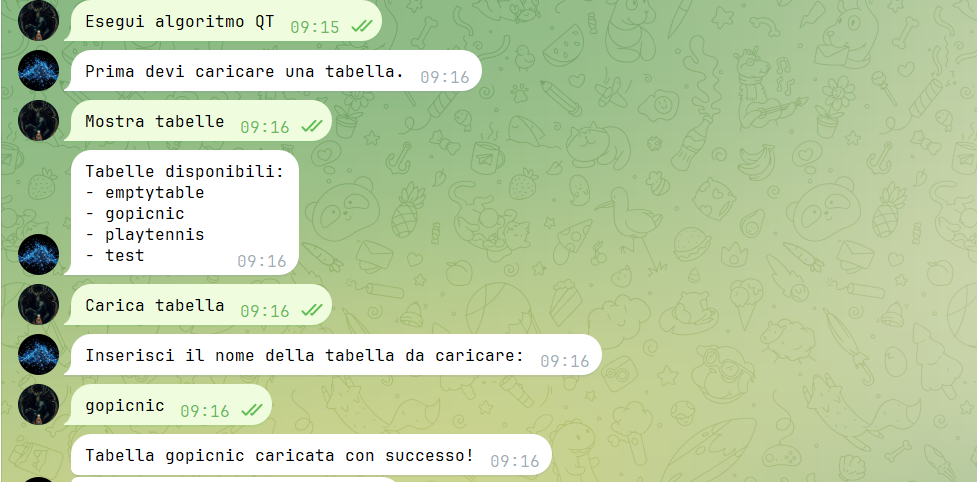
\includegraphics[width=0.45\textwidth]{images/caricamento tabella.png}
    }
    \hfill
    \subfloat[Risultato dell'esecuzione]{
        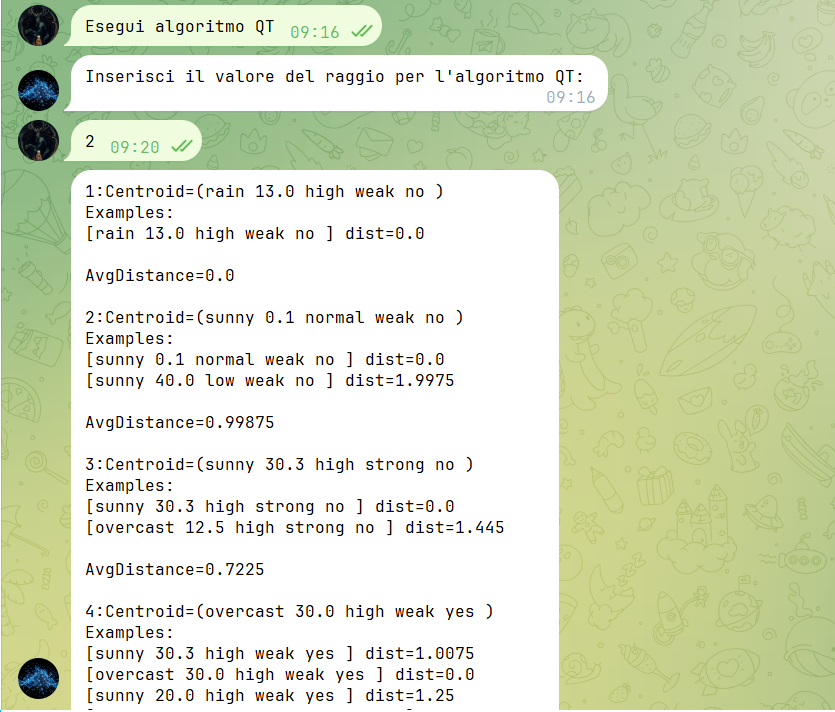
\includegraphics[width=0.45\textwidth]{images/esecuzione algoritmo.png}
    }
    \caption{Processo di esecuzione dell'algoritmo QT}
\end{figure}

\subsection{Salvare i risultati}

Una volta eseguito l'algoritmo QT, il bot permetterà di salvare il risultato dell'esecuzione in un file \texttt{.dmp}, in maniera molto simile a come avvenivna nel progetto base, all'interno della cartella \texttt{results}, presente nella cartella principale del progetto esteso. 

\image{images/cartella results.png}{Posizione cartella results}{results}

Chiaramente per eseguire tale operazione, è necessario premere il pulsante \texttt{Salva Risultati}. 

\image{images/salva risultati.png}{Opzione di salvataggio dei risultati}{salvarisultati}

\subsection{Caricare un risultato precedente}

Qualora si voglia caricare un risultato precedentemente salvato, è possibile farlo premendo il pulsante \texttt{Carica Risultati}. 

\image{images/carica risultati.png}{Opzione di caricamento dei risultati}{caricarisultati}

Il bot non chiederà direttamente di inserire il nome del file da caricare ma, dato che il nome del file \texttt{.dmp} è costruito in modo da contenere le informazioni relative al raggio e alla tabella utilizzata per l'esecuzione dell'algoritmo QT, il bot chiederà di inserire il raggio e  la tabella da ritrovare. 

Se il file \texttt{.dmp} esiste, il bot risponderà restituendo il risultato dell'esecuzione in questione. 

\image{images/risultato caaricamento .png}{Risultato del caricamento di un file .dmp}{riscaricamento}

\subsection{Ritono al menù principale}

Qualora si voglia far ripartire il bot dalla schermata iniziale, è possibile farlo premendo il pulsante \texttt{Torna al menù principale}.

Una volta premuto il pulsante, il bot risponderà con un messaggio di benvenuto, come quello mostrato alla fine della sezione \ref{Schermata iniziale}.

